\documentclass[a4paper,10.0pt,twoside]{npr}

\usepackage{multicol,graphicx,lastpage,footmisc,fancyhdr,paralist,
tabularx,array,booktabs,caption,multirow,upgreek,mathrsfs,gensymb,color}
\usepackage[fancyhdr,space,fntef,fontset=ubuntu]{ctex}
\usepackage{amssymb,bm,mathrsfs,bbm,amscd}
\usepackage{flushend,cuted}
\usepackage{refcount}
\usepackage{savesym}
\usepackage{textcomp}
\usepackage[tbtags]{amsmath}  %
\savesymbol{iint}
\usepackage{amstext} %数学宏包文本命令
\usepackage{balance} %版心底部对齐

\flushbottom      %版心底部对齐
\setcounter{section}{0}
\begin{document}
%\begin{CJK*}{GBK}{\song}{\wuhao}{\rm}

%___________________________________________________________________________________
\def\rd{{\rm d}}

\newcommand{\RM}{\ensuremath{\mathrm}}   %正体 既可用于文本模式也可用于数学模式
\newcommand{\dif}{\mathrm{d}}  %直立体d
\newcommand{\me}{\mathrm{e}}  %直立体e
\newcommand{\mi}{\mathrm{i}}  %直立体i
\newcommand{\mj}{\mathrm{j}}  %直立体j
\newcommand{\afrac}[2]{\dfrac{\,#1\,}{\,#2\,}}  %略长分数线
\newcommand{\nn}{\nonumber}  %公式无编号
\newcommand{\nt}{\noindent}
\newcommand{\OO}{~\text{。}}
\newcommand{\PP}{~\text{,}}
\newcommand{\OP}{~\text{;}}
\newcommand{\LT}{\left}
\newcommand{\RT}{\right}

%___________________________________________________________________________________

\balance
\fancypagestyle{myfoot}
{%
\fancyhf{}
\fancyhead[c]{\wuhao\song 高~等~核~物~理~实~验}
\renewcommand{\headrule}{\vskip 2pt
\hrule height0.4pt width\headwidth \vskip1pt
\hrule height0.4pt width\headwidth \vskip-1.8pt}
}%
\thispagestyle{myfoot}

%%%%%%%%%%%%%%%%%%%%%%%%%%%%%%%%%%%%%%%%%%%%%%%%%%%%%
%    奇偶页眉
%%%%%%%%%%%%%%%%%%%%%%%%%%%%%%%%%%%%%%%%%%%%%%%%%%%%%
\pagestyle{fancy}
\fancyhead{}
\fancyhead[ce]{\xiaowu\song \hspace{0.5em}高~等~核~物~理~实~验}
%\fancyhead[ro,le]{\xiaowuhao \hspace{0.5em}\textbf{\textperiodcentered}\;\thepage\;\textbf{\textperiodcentered}\hspace{0.5em}}
%\fancyhead[ce]{\xiaowu\song 粒~子~物~理~与~原~子~核~物~理~专~题~实~验}
%\fancyhead[re]{\xiaowu\song \hspace{0.5em}第\;31\;卷\hspace{0.5em}}
\fancyfoot[ce,co]{}
\renewcommand{\headrule}{\vskip 2pt
\hrule height0.4pt width\headwidth}


\setcounter{page}{001}%
\fancyhead[co]{\xiaowuhao\song  乔颢:正电子在物质中的湮没寿命}    %奇页页眉
\begin{center}
\title{%
\xiaoerhao \bf  %章标题为两行时改为 \exiaoer
正电子在物质中的湮没寿命\\[-5mm]}
\maketitle
\large \fs
乔颢$^{^1}$\\[2mm]

\xiaowu \song
1. 北京大学物理学院,海淀区 北京 100871;\\[4mm]

 
\footnotetext[0]{{\bf 作者简介:}~~\begin{minipage}[t][4.2mm]{149mm}\song
乔颢,E-mail: i@catofes.com
\end{minipage} }
%\footnotetext[0]{{\bf 通信作者:}\song ~~E-mail: xxx@xxx.xxx }%通信作者为第一作者时不要此项

\parbox{158mm} {
\zywu{\bf 摘要:}~~\fs
本试验使用符合方法测量正电子在物质中的湮灭时间,测量得到正电子的长寿命约为0.385ns,短寿命约为0.222ns。

{\bf 关键词:}~~\fs 正电子,湮灭,符合}\\
\end{center}
%%%%6.正文
\vspace{5mm}
%%%%6.正文
\setcounter{section}{0}
\begin{multicols}{2}
%----------------
%____________________________________________________________________________
%%%%以上请不要改动%%%%%%%%%%%%%%%%%%%%%%%%%%%%%%%%%%%%%%%%%%%%

\section{实验原理}    %1
\vspace*{-1mm}
\song\wuhao
\subsection{正电子的湮灭寿命}
正电子是电子的反粒子,除电荷和磁矩符合不同外,其他特性与电子相同。当正电子与负电子相遇时发生“湮灭”,它们的总能量以电磁辐射能的形式发射出来,湮灭过程的绝大多数是发射两个能量相等、方向相反的$\gamma$光子。
放射源发射的正电子,通常具有几百keV的动能,进入物质以后与物质的分子原子相碰撞,很快损失它的动能,在极端时间之内(~10ps)与物质达到热平衡,然后继续在物质中运动,直到与负电子相遇发生湮灭。正电子从产生到湮灭的时间间隔,称为正电子在物质中的湮灭寿命。它由物质的物理、化学性质决定,在金属中,正电子的寿命约为100ps到500ps。

\subsection{测量正电子寿命的实验原理}

测量正电子的寿命时,正电子源通常用$^{22}$Na,它的衰变纲图如图1所示。$^{22}$Na 发生$\beta^{+}$衰变时放出正电子e$^{+}$,$^{22}$Na转变到$^{22}$Ne的激发态,此激发态的激发能为1280keV,寿命约为$3\times10^{-12}$秒,通过发射1275keV的$\gamma$射线退激到$^{22}$Ne的基态。在时间谱仪的分辨时间为$10^{-10}$秒的情况下,可以认为上述核转变过程中发射e$^{+}$和$\gamma$是同时进行的。在测量正电子寿命时,1275keV$\gamma$射线可作为e$^{+}$产生的时标信号;而e$^{+}$湮没时放出的两个511keV$\gamma$光子作为正电子湮没的时标信号。测量正电子产生和湮没的时标信号之间的时差,即可得正电子寿命。
\begin{center}
   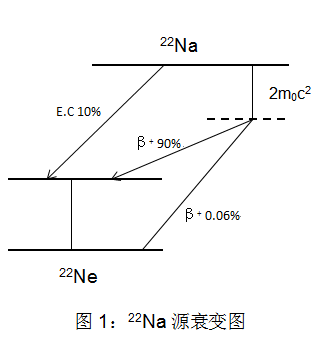
\includegraphics[width=0.45\textwidth]{1.png}
\\
\xiaowu\song 图~1\begin{minipage}[t]{75mm} \quad $^{22}$Na衰变纲图\\[-1mm]\wuhao
\end{minipage}
\end{center}

\section{实验装置和原理}
多道时间谱仪,是测量两个时间关联事件之间的短时间间隔装置。它可用来测量正电子在物质中的湮没寿命、粒子飞行时间谱、核激发态寿命等。它分析的时间从$10^{-6}$到$10^{-10}$秒。

\begin{center}
   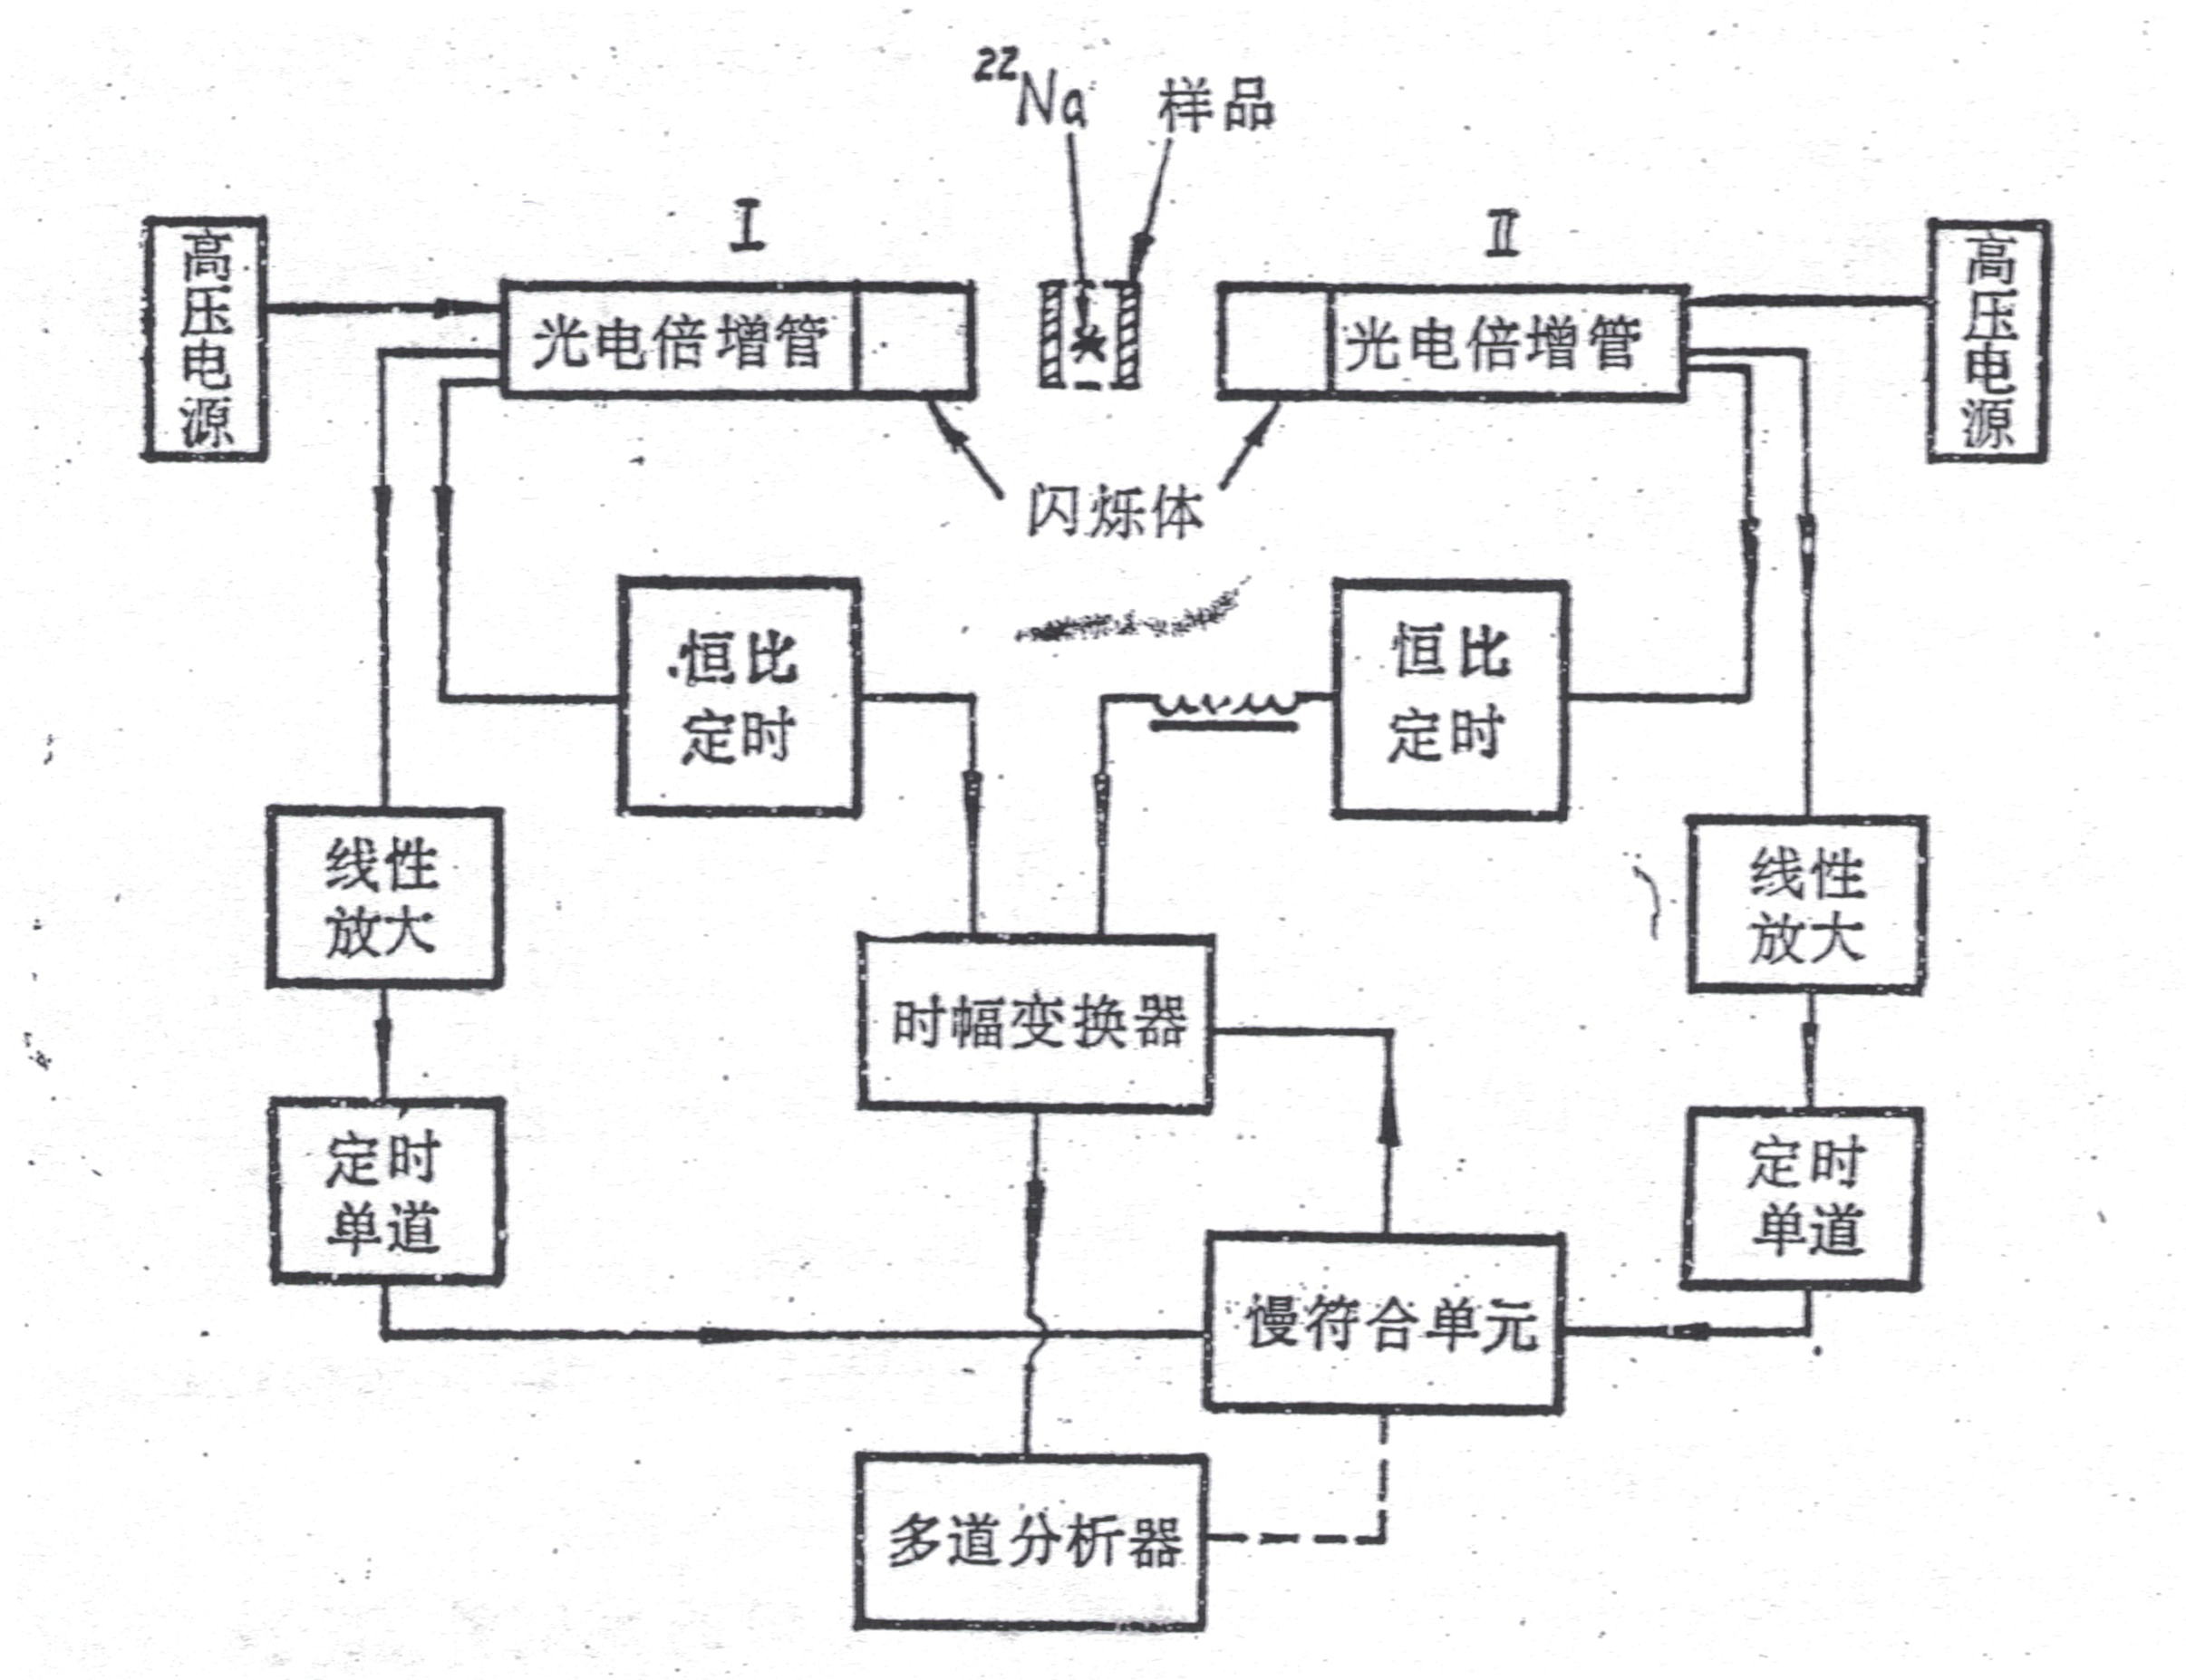
\includegraphics[width=0.45\textwidth]{2.png}
\\
\xiaowu\song 图~2\begin{minipage}[t]{75mm} \quad $^{22}$多道时间谱仪\\[-1mm]\wuhao
\end{minipage}
\end{center}

该谱仪的组成如图2所示。它通过时间幅度变换器把关联事件的时间间隔变成电压脉冲幅度,然后由多道分析器测量幅度分布谱,从而得到关联事件的时间分布谱。

\subsection{探头}
由快塑料闪烁体和快光电倍增管组成,用来探测关联事件。光电倍增管的阳极负信号作为事件发生的时标信号,直接耦合到时间道(快道)的定时甄别器的输入端;光电倍增管的打拿极作为能量的选择信号,经射极跟随器输出到能量道(慢道)。由图2可以看到,总共有两个探头,与每个探头相连的其他部分是左右对称的。
\subsection{快道}
又称时间选择道,从时间关系上选出来关联事件对$\gamma_1\gamma_2$,同时把$\gamma_1$与$\gamma_2$之间的时间差转换为脉冲幅度。图2中,由探头I的阳极送到I道恒比定时器的信号,经过甄别、成形,产生的起始事件$\gamma_1$的时标信号,然后送到时幅变换器的起始输入端,启动时幅变换器开始变换。探头II的阳极信号经过II道恒比定时器同样的处理后送到时幅变换器的终止端,使变换终止,变换得到的脉冲数目代表选出的关联事件对数目。
\subsection{慢道}
又称能量选择道,是为了减少偶然符合本底和改善分辨时间,进一步选出关联的事件。
\subsection{快慢符合}将慢符合单元的输出信号去开时幅变换器的选通门,使时幅变换
器输出的脉冲得以输出。这样的时幅变换器输出的信号表示经过事件选择和能量选择的关联事件。

\section{实验内容和结果}

按照图示连接线路,放上$^{60}$Co源,调节两路单道的阈值和道宽,使得康普顿平台位于约800道处。然后将单道的输出信号展宽后作为反符合信号输入多道中,选择能量窗口使得$\Delta V/V\approx 45\%$左右。

两路调节完成后就可以用延时插件对时幅转换器做时间刻度了。数据图如下所示:

\begin{center}
   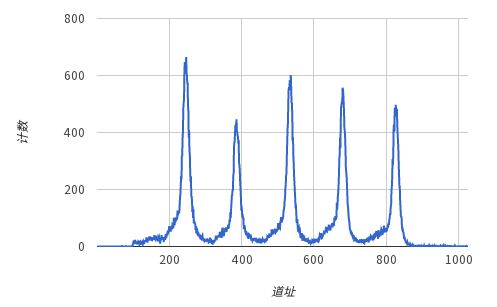
\includegraphics[width=0.45\textwidth]{3.png}
\\
\xiaowu\song 图~3\begin{minipage}[t]{75mm} \quad 时间刻度。图中的5个峰分别对于16ns,20ns,24ns,28ns,32ns。\\[-1mm]\wuhao
\end{minipage}
\end{center}

利用寻峰算法得到峰位后可以拟合得到时间和道址的信息,如下图所示。拟合得到的结果为 $$t = 0.028 \times channel + 9.329$$

\begin{center}
   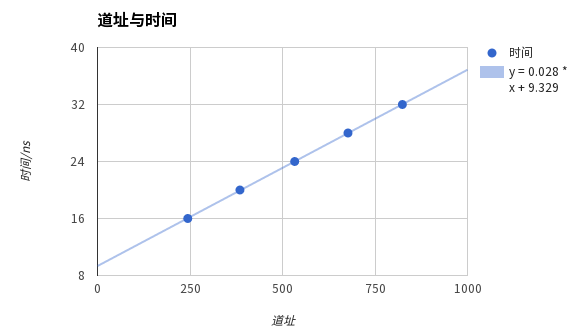
\includegraphics[width=0.45\textwidth]{4.png}
\\
\xiaowu\song 图~4\begin{minipage}[t]{75mm} \quad 时间刻度拟合结果\\[-1mm]\wuhao
\end{minipage}
\end{center}

随后是测量能选道(慢道)的$N_C-t_d$曲线。如下图所示:

\begin{center}
   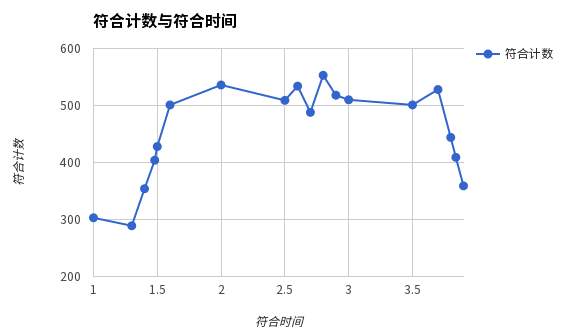
\includegraphics[width=0.45\textwidth]{5.png}
\\
\xiaowu\song 图~5\begin{minipage}[t]{75mm} \quad $N_C-t_d$曲线,符合时间单位为$\mu s$\\[-1mm]\wuhao
\end{minipage}
\end{center}

从图中看出在1.5$\mu s$到3.8$\mu s$之间计数基本是一个平台,所以可以取中间位置也就是2.66$\mu s$。

接下来是对时间分辨率的测定。取延时时间为16ns时候,对比有无能选时候时间分辨作比较,可以得到在没有能选时候分辨率为8.1\%,在加入能选之后分辨率则降至5.1\%,可以看出加入能选能够有效提高分辨精度。具体的时间分辨可以计算出来,没有能选时候半高宽为19.8道,对应的时间为0.55ns,在加入能选之后半高宽为14.6,对应的时间为0.41ns。虽然加入了能选提高了很多时间分辨率,但是计数率有着明显的下降,所以测量时间就需要增加。

最后就可以用这一套仪器测量正电子的寿命了。选取能量窗口分别为1275以及511keV的两个区域,由此测量得到的正点子湮灭时间谱如下图所示:

\begin{center}
   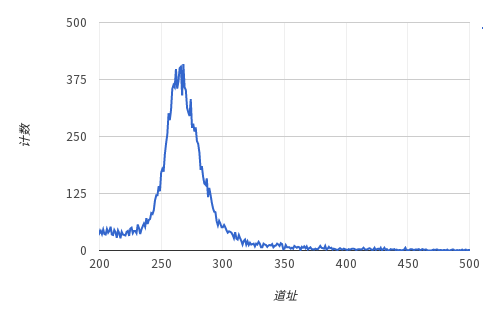
\includegraphics[width=0.45\textwidth]{6.png}
\\
\xiaowu\song 图~6\begin{minipage}[t]{75mm} \quad 正点子湮灭时间谱。\\[-1mm]\wuhao
\end{minipage}
\end{center}

然后就可以计算寿命了。首先计算长寿命,此时计数和时间的关系为:

$$Y_1(t) \approx N_{01} e^{-\lambda_1 t}$$

取对数则有:

$$ \ln Y_1(t) = \ln N_{01} - \lambda_1 t$$

选取从第300道到310道的数据进行拟合可以得到$\ln N_{01} = 35.87$,$\lambda_1 = -1.799$, 即长寿命为$\ln 2 /1.799=0.385ns$。

然后计算短寿命,有

$$ \ln (Y(t) -Y_1(t)) = \ln N_{02} -\lambda_2 t$$

带入$Y_1$的结果可以拟合得到$\lambda_2  = -3.119$,计算可以得到短寿命为$\ln 2 /3.119=0.222ns$。


\section{参考文献}

\noindent
[1] Peking Unviersity, Fudan University \ Nuclear Experment
\ Nuclear Publishing House, 1989 (in Chinese)

\noindent
 (北京大学,复旦大学.\ 原子核实验\ 原子能出版社,\ 1989)

\end{multicols}

\newpage

\clearpage
%\end{CJK*}
\end{document}

